\chapter{基于Hadoop的MapReduce程序设计}
\label{chap:3}

\section{Web访问日志分析程序设计}
\subsection{程序应用场景}
随着互联网的高速发展,各种Web2.0网站、电子商务网站创造了前所未有的访问记录,各种大型网络游戏不断刷新着在线用户数峰值,与此同时这些大型系统都记录下了海量的运行日志。挖掘出日志中蕴藏的信息来改进用户体验提升服务质量是非常有价值的。本程序利用MapReduce框架,利用分布式集群处理访问日志计算PV,可以解决传统生产环境中单机处理Web访问日志速度过慢的问题。

\subsection{程序实现过程}
本程序基于Hadoop 1.0.1,利用MapReduce思想进行程序开发。MapReduce思想十分简单,首先将所有的数据分发到各个集群上,并在集群执行Map函数,之后将Map结果合并并交给reduce做进一步的计算,详见本文第\ref{chap:2}章。

根据MapReduce思想,根据实际需求,本程序运行流程图如图\ref{fig:程序流程图}所示:

\begin{figure}[h]
 \centering
 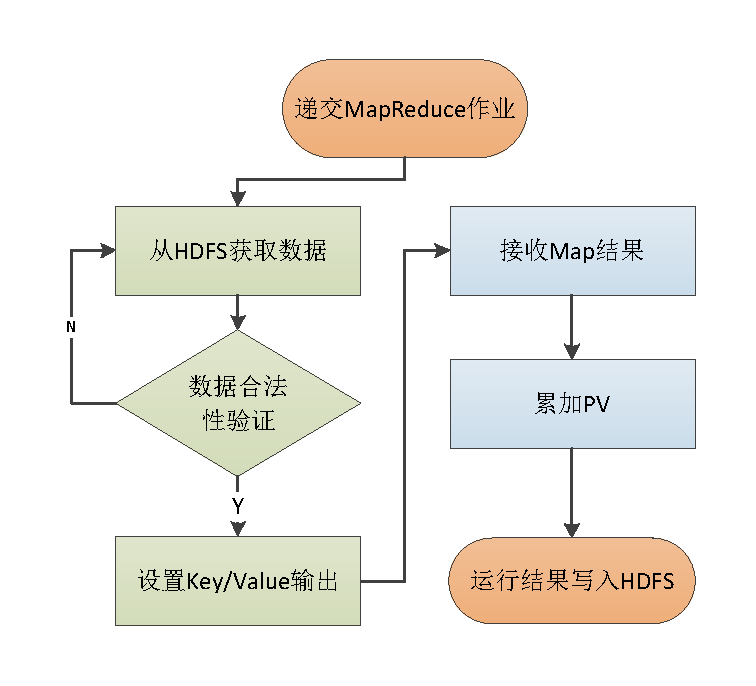
\includegraphics[width=0.7\textwidth]{程序流程图}
 \caption{程序流程图}
 \label{fig:程序流程图}
\end{figure}

Map函数的功能为:从HDFS上获取日志文件,文件每一行作为一个输入,Mapper在读取行之后,验证其访问的有效性,之后设置“pv”作为Mapper的key,1作为值,将Map结果输出。

Reduce函数的功能为:从Map端接收合并好的Key/Value对,将key所对应的Value的值相加,得到PV值,将新的Key/Value对输出。

\subsection{程序运行环境}
Hadoop依赖SSH和JDK,具有很高的通用性,但一般情况下,为了整体集群的效率,操作系统一般选用Linux,使用Sun JDK,本程序的开发运行环境具体如下:

实验机器配置:

CPU:Pentium(R) Dual-Core  CPU E5800 @ 3.20GHz

内存:2G DDR2 800

硬盘:Seagate 320G 7200RPM

操作系统:CentOS\_6.2\_x64
  
CentOS是RedHat的开源版本,具有了RedHat的一切特性并有着稳定的社区支持,以其高效和稳定著称,是理想的Hadoop宿主操作系统。6.2是其最新稳定版。本文中所使用的CentOS为netinstall版,这种方式安装出来的CentOS体积最小,软件包最新,服务数量最少,运行速度最快,且不损失任何系统稳定性。

JDK:Sun JDK 1.6.0\_31

Java Development Kit (JDK) 是Sun公司针对Java开发人员发布的免费软件开发工具包(SDK,Software development kit)。自从Java推出以来,Sun JDK已经成为使用最广泛的Java SDK。1.6.0\_31是其最新稳定版。

Hadoop 1.0.1

Hadoop是Apache社区下的开源软件,1.0.1是其最新稳定版。

编程语言:Java、Python 2.6

编程语言的差异会对程序的运行效率产生至关重要的影响,本实验选用Java、Python两种最常见的解释性编程语言,便于后期性能对比。


\section{程序开发与实现}
\subsection{原生Java的实现}
Hadoop使用Java语言实现,其自身提供了一套完整的Java类库,使用起来十分方便。

首先,创建一个Java文件,在文件头部定义package名称,引入相关类库之后就可以开始编写Mapreduce程序了,程序中需要在Java包内定一个一个Public类pv,运行时,将类名作为参数传入Hadoop。pv类里定义Map和Reduce类和一个main函数:TokenizerMapper继承Mapper类,IntSumReducer继承Reducer类,main函数里指定运行的Map和Reduce类名、和数据类型,其各部分具体功能如下:

TokenizerMapper定义两个private变量,用于存储Key/Value的值。之后定义一个map函数,判断读入的数据的合法性,若合法,则给value赋值1,反之赋值0。

IntSumReducer定义一个变量,用于存储最终pv的值。之后定一个一个函数reducer,将Map传入的结果累加。最后输出Key和pv值。

main函数中实例化Hadoop的配置类、和Job类,并给job类的各项属性赋值。

编写完毕之后,应对程序进行调试,Hadoop为Eclipse提供了完整的调试插件,但由于其配置复杂且超出了本文讨论范围,在此不详细给出。

其在Hadoop中的运行流程如图\ref{fig:运行过程-java}所示:

\begin{figure}[h]
 \centering
 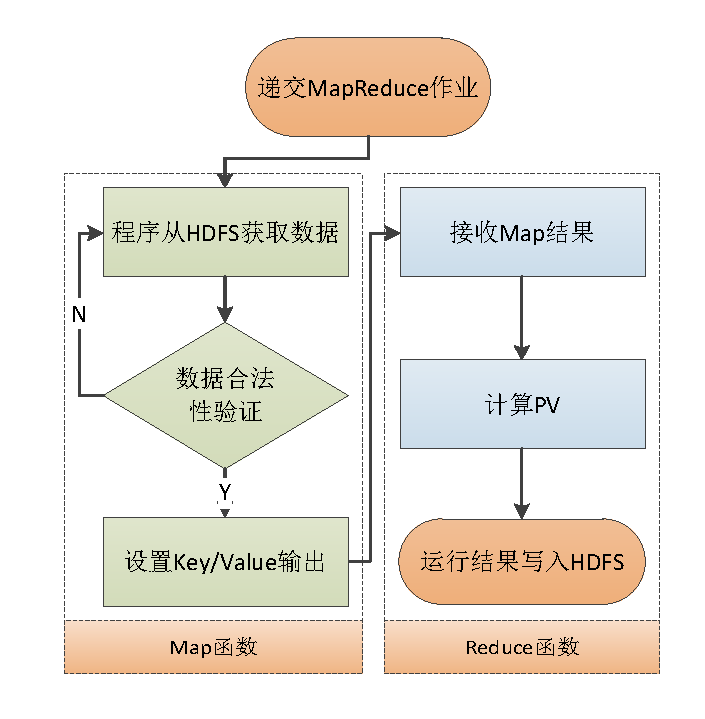
\includegraphics[width=0.7\textwidth]{运行过程-java}
 \caption{运行过程-java}
 \label{fig:运行过程-java}
\end{figure}

至此,Web日志处理的Java程序就实现了。

\subsection{基于Streaming的Python实现}
Hadoop在支持原生Java的同时也对外提供了Streaming方法,该方法把HDFS中的文件读写转化成文件流,传入外部程序处理,使得Hadoop具有处理非Java编写的程序的能力。本文选用了和Java及其类似的解释性编程语言Python,便于后期的性能测试对比。

新建文件Mapper.py,文件首部向系统声明文件执行类型为python,又因程序使用std I/O并分割字符串,所以在头部引用sys和itemgetter。之后使用for循环语句从sys.stdin读取数据,并判断其合法性,若合法,则给value赋值1,反之赋值0,最后使用print输出Key/Value对,并以一个缩进符号分割开来。

新建文件Reducer.py,文件首部和引用于Mapper.py相同,定义存储pv值的变量sum,使用for循环从sys.stdin读取Mapper中生成的文件流,使用itemgetter分割Key/Value对到对应的变量,将pv值累加。最后使用print输出Key和pv值。

由于Streaming使用std I/O,使得其调试非常简单,用户可以直接在本机使用cat命令通过Unix管道即可进行简单的的调试。运行命令cat 10.log | ./mapper.py即可查看Map的结果。

在Hadoop中运行时,应向hadoop指定map文件和reduce文件,并使用file命令将map/reduce程序分发到各节点。

其在Hadoop中的运行流程如图\ref{fig:运行过程-streaming}所示:

\begin{figure}[h]
 \centering
 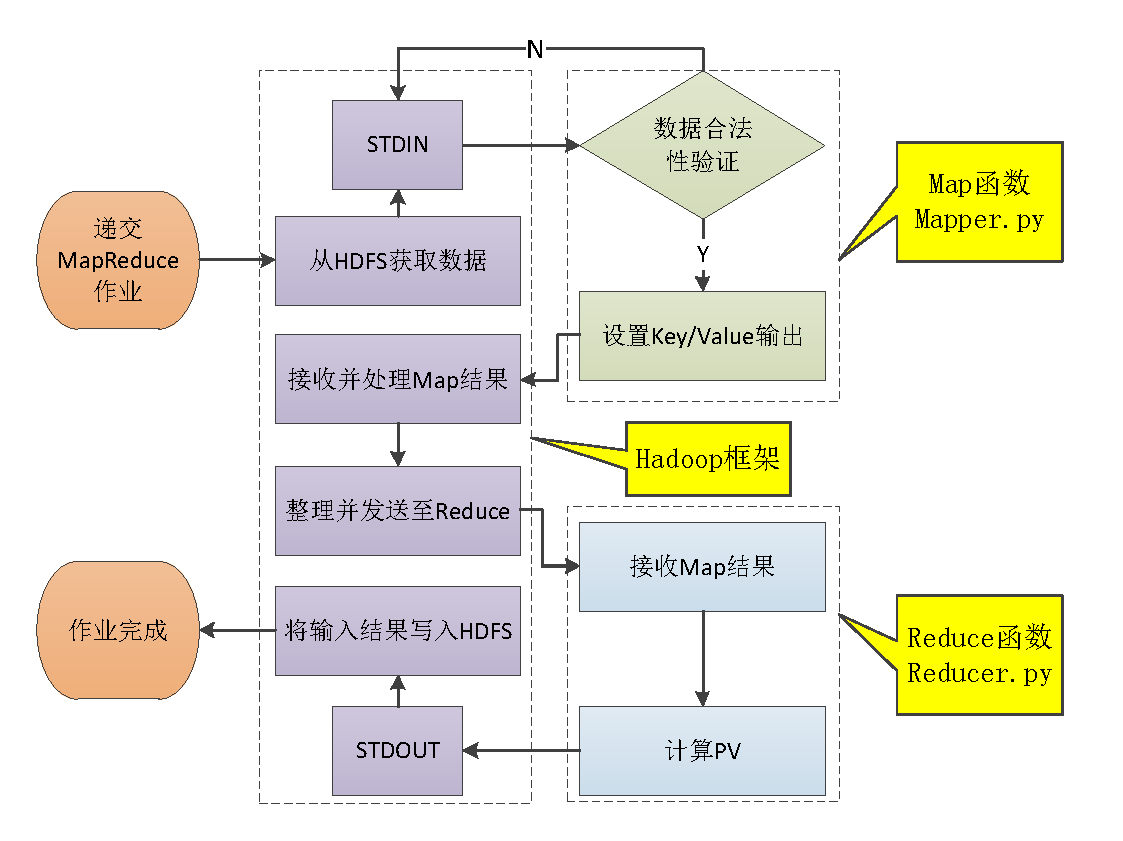
\includegraphics[width=0.7\textwidth]{运行过程-streaming}
 \caption{运行过程-streaming}
 \label{fig:运行过程-streaming}
\end{figure}


至此,Web日志处理的Python程序就实现了。

\section{实现效果及性能测试}
\subsection{测试数据及方法}
为了验证本程序的正确性和运行效率,笔者使用了9组数据,测试数据为基数为10到100,000,000,增量为十倍,共8组清洗过的有效合法日志,日志取自实际生产环境服务器,具有一定的参考价值。所有测试数据均存放在采用Hadoop默认配置的HDFS上。

测试环境为伪分布式的单机Hadoop节点,Java和Python程序的运行均使用Hadoop默认参数执行,测试过程中,使用sar对系统资源进行监测,测试结束后,收集运行日志进行更进一步的分析。


\subsection{基于原生Java的实现及性能测试}
本实验中Java程序均使用Sun\_JDK\_1.6.0\_31编译并打包,Java程序上传到服务器上之后,执行命令

\begin{verbatim}
hadoop jar pv.jar test.pv input/100.log output/java/100
\end{verbatim}

其中pv.jar为打包后的程序,test.pv为程序中所对应的包及类,input/100.log为HDFS上的日志文件, output/java/100为输出目录。

命令执行后,终端会实时跟踪程序运行情况,用户也可以通过网页查看当前程序的运行状况。程序执行完毕之后,Hadoop会将程序运行信息输出至终端,程序运行结果保存在指定的HDFS目录下,用户可以运行以下命令查看运行结果。
\begin{verbatim}
hadoop dfs -cat output/java/100/part-r-00000
\end{verbatim}
在本实验中,所用测试数据是提前使用工具处理好的数据,目的在于验证程序的准确性并分析对比其运行时间。具体运行结果和运行时间如下表\ref{tab:java1}和表\ref{tab:java2}:

\begin{table}[htbp]
 \caption{\label{tab:java}Java程序的Map、Reduce数量及其运行时间}
 \centering
 \begin{tabular}{cccccc}
  \toprule
  Log大小 & Map & Reduce & Map运行 & Reduce运行 & 总时间\\
  (行) & 数量 & 数量 & 时间(ms) & 时间(ms) & 时间(ms)\\
  \midrule
  100 & 1 & 1 & 460 & 1,410 & 1,870\\
  1,000 & 1 & 1 & 240 & 1,420 & 1,660\\
  10,000 & 1 & 1 & 770 & 1,260 & 2,030\\
  100,000 & 1 & 1 & 2,310 & 1,170 & 3,480\\
  1,000,000 & 7 & 1 & 17,400 & 1,510 & 18,910\\
  10,000,000 & 67 & 1 & 164,750 & 5,400 & 170,150\\
  100,000,000 & 648 & 1 & 1,580,020 & 14,790 & 1,594,810\\
  \bottomrule
 \end{tabular}
\end{table}


\begin{table}[htbp]
 \caption{\label{tab:java}Java程序的本地缓存相关数据统计}
 \centering
 \begin{tabular}{cccccc}
  \toprule
  Log大小 & 本地写入 & 本地读取 & Shuffle & Combine & Combine\\
  (行) & (byte) & (byte) & (byte) &  Input & Output\\
  \midrule
  100 & 42,951 & 15 & 0 & 100 & 1\\
  1,000 & 42,955 & 15 & 0 & 1,000 & 1\\
  10,000 & 42,959 & 15 & 0 & 10,000 & 1\\
  100,000 & 42,963 & 15 & 15 & 100,000 & 1\\
  1,000,000 & 172,015 & 69 & 105 & 1,000,000 & 7\\
  10,000,000 & 1,462,756 & 609 & 990 & 10,000,000 & 67\\
  100,000,000 & 13,963,723 & 5,838 & 9,705 & 100,000,000 & 648\\
  \bottomrule
 \end{tabular}
\end{table}

\subsection{基于Streaming的Python实现及其性能测试}

本实验中的Python程序均使用CentOS自带的Python 2.6.6解析,在Hadoop端使用默认参数运行Streaming。

Python程序上传到服务器上之后,执行命令

\begin{verbatim}
hadoop jar $HADOOP_HOME/contrib/streaming/hadoop-streaming-1.0.1.jar \
-file mapper.py -mapper mapper.py \
-file reducer.py -reducer reducer.py \
-input input/100.log -output output/python/100
\end{verbatim}

其中\$HADOOP\_HOME/contrib/streaming/hadoop\-streaming\-1.0.1.jar为Hadoop内置的Streaming类,\-file命令将程序分发到各节点,\-mapper和\-reducer命令分别制定mapper.py和reducer.py为Mapper和Reducer,input/100.log为HDFS上的日志文件, output/python/100为输出目录。

命令执行后,同原生Java一样,终端会实时跟踪程序运行情况,用户也可以通过网页查看当前程序的运行状况。程序执行完毕之后,Hadoop会将程序运行信息输出至终端,程序运行结果保存在指定的HDFS目录下用户可以运行一下命令查看运行结果。

\begin{verbatim}
hadoop dfs -cat output/python/100/part-r-00000
\end{verbatim}

同上一小节,在本实验中,所用测试数据是提前使用工具处理好的数据,目的在于验证程序的准确性并分析对比其运行时间。

与原生Java运行效果相比,Streaming的处理时间比Java长,在下一章里,本文会对这一现象进行详细的分析和说明。

具体运行结果和运行时间如下表\ref{tab:python1}和表\ref{tab:python2}:

\begin{table}[htbp]
 \caption{\label{tab:python1}Python程序的Map、Reduce数量及其运行时间}
 \centering
 \begin{tabular}{cccccc}
  \toprule
  Log大小 & Map & Reduce & Map运行 & Reduce运行 & 总时间\\
  (行) & 数量 & 数量 & 时间(ms) & 时间(ms) & 时间(ms)\\
  \midrule
  100 & 2 & 1 & 640 & 2,290 & 2,930\\
  1,000 & 2 & 1 & 800 & 1,750 & 2,550\\
  10,000 & 2 & 1 & 1,210 & 2,300 & 3,510\\
  100,000 & 2 & 1 & 2,830 & 2,060 & 4,890\\
  1,000,000 & 7 & 1 & 20,310 & 3,250 & 23,560\\
  10,000,000 & 67 & 1 & 191,800 & 30,870 & 222,670\\
  100,000,000 & 648 & 1 & 1,832,430 & 283,340 & 2,115,770\\
  \bottomrule
 \end{tabular}
\end{table}


\begin{table}[htbp]
 \caption{\label{tab:python2}Python程序的本地缓存相关数据统计}
 \centering
 \begin{tabular}{cccccc}
  \toprule
  Log大小 & 本地写入 & 本地读取 & Shuffle & Combine & Combine\\
  (行) & (byte) & (byte) & (byte) &  Input & Output\\
  \midrule
  100 & 67,330 & 706 & 300 & 0 & 0\\
  1,000 & 79,936 & 7,006 & 3,541 & 0 & 0\\
  10,000 & 205,942 & 70,006 & 70,012 & 0 & 0\\
  100,000 & 1,465,948 & 700,006 & 353,632 & 0 & 0\\
  1,000,000 & 14,175,921 & 7,000,006 & 6,271,973 & 0 & 0\\
  10,000,000 & 141,495,890 & 70,000,006 & 69,224,334 & 0 & 0\\
  100,000,000 & 1,414,279,852 & 700,000,054 & 699,780,106 & 0 & 0\\
  \bottomrule
 \end{tabular}
\end{table}

\section{本章小结}
本章以Web访问日志程序开发为例,分别介绍了在Hadoop下的两种程序开发模式:原生Java和Streaming,并对进行了正确性验证,证明了MapReduce框架的正确性和可行性,并收集了相关有价值的Counter数据。在下一章里,本文会根据本章第三节所摘录的测试结果做以分析和说明。